\documentclass[tikz,border=5pt]{standalone}
\usepackage{pgfplots}
\pgfplotsset{compat=1.18}
\usepackage{fontspec}
\setsansfont{SourceSansPro}[
  Path = /usr/local/texlive/2024/texmf-dist/fonts/opentype/adobe/sourcesanspro/,
  UprightFont = SourceSansPro-Regular.otf,
  BoldFont = SourceSansPro-Bold.otf,
  ItalicFont = SourceSansPro-RegularIt.otf,
  BoldItalicFont = SourceSansPro-BoldIt.otf,
  Scale = 1.0
]
\usetikzlibrary{positioning}
\usepackage{xcolor}
\definecolor{primaryblue}{HTML}{012169}
\definecolor{primarygold}{HTML}{B9975B}
\definecolor{highlightyellow}{HTML}{F2A900}
\definecolor{lightbg}{HTML}{E8EDF5}
\definecolor{jet}{HTML}{1A1A1A}
\definecolor{positivegreen}{HTML}{15803D}
\definecolor{negativered}{HTML}{B91C1C}
\begin{document}
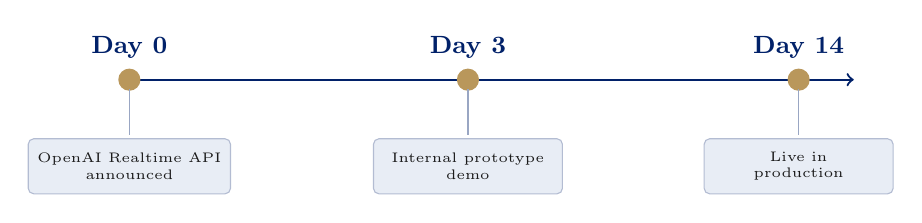
\begin{tikzpicture}[
  desc/.style={draw=primaryblue!30, fill=lightbg, rounded corners=2pt,
               minimum width=2.4cm, minimum height=0.7cm,
               font=\tiny, align=center, text=jet}
]
  % Timeline axis
  \draw[->, thick, color=primaryblue] (0,0) -- (9.2,0);

  % Day 0
  \fill[primarygold] (0,0) circle (4pt);
  \node[font=\small\bfseries\color{primaryblue}, above=4pt] at (0,0) {Day 0};
  \draw[primaryblue!40, thin] (0,-0.12) -- (0,-0.7);
  \node[desc] at (0,-1.1) {OpenAI Realtime API\\announced};

  % Day 3
  \fill[primarygold] (4.3,0) circle (4pt);
  \node[font=\small\bfseries\color{primaryblue}, above=4pt] at (4.3,0) {Day 3};
  \draw[primaryblue!40, thin] (4.3,-0.12) -- (4.3,-0.7);
  \node[desc] at (4.3,-1.1) {Internal prototype\\demo};

  % Day 14
  \fill[primarygold] (8.5,0) circle (4pt);
  \node[font=\small\bfseries\color{primaryblue}, above=4pt] at (8.5,0) {Day 14};
  \draw[primaryblue!40, thin] (8.5,-0.12) -- (8.5,-0.7);
  \node[desc] at (8.5,-1.1) {Live in\\production};
\end{tikzpicture}
\end{document}
